\documentclass[a4paper,12pt]{article}
\usepackage[indonesian]{babel}
\usepackage{graphicx}
\usepackage{multirow}
\usepackage{enumitem}
\usepackage{listings}
\usepackage{wrapfig}
\usepackage[T1]{fontenc}
\usepackage{inconsolata}
\usepackage{lipsum}
\usepackage{adjustbox}


\usepackage{color}
\usepackage[table]{xcolor}
\definecolor{lightgray}{rgb}{0.95, 0.95, 0.95}
\definecolor{darkgray}{rgb}{0.4, 0.4, 0.4}
%\definecolor{purple}{rgb}{0.65, 0.12, 0.82}
\definecolor{editorGray}{rgb}{0.95, 0.95, 0.95}
\definecolor{editorOcher}{rgb}{1, 0.5, 0} % #FF7F00 -> rgb(239, 169, 0)
\definecolor{editorGreen}{rgb}{0, 0.5, 0} % #007C00 -> rgb(0, 124, 0)
\definecolor{orange}{rgb}{1,0.45,0.13}		
\definecolor{olive}{rgb}{0.17,0.59,0.20}
\definecolor{brown}{rgb}{0.69,0.31,0.31}
\definecolor{purple}{rgb}{0.38,0.18,0.81}
\definecolor{lightblue}{rgb}{0.1,0.57,0.7}
\definecolor{lightred}{rgb}{1,0.4,0.5}
\usepackage{upquote}
\usepackage{listings}
% CSS
\lstdefinelanguage{CSS}{
  keywords={color,background-image:,margin,padding,font,weight,display,position,top,left,right,bottom,list,style,border,size,white,space,min,width, transition:, transform:, transition-property, transition-duration, transition-timing-function},	
  sensitive=true,
  morecomment=[l]{//},
  morecomment=[s]{/*}{*/},
  morestring=[b]',
  morestring=[b]",
  alsoletter={:},
  alsodigit={-}
}

% JavaScript
\lstdefinelanguage{JavaScript}{
  morekeywords={typeof, new, true, false, catch, function, return, null, catch, switch, var, if, in, while, do, else, case, break},
  morecomment=[s]{/*}{*/},
  morecomment=[l]//,
  morestring=[b]",
  morestring=[b]'
}

\lstdefinelanguage{HTML5}{
  language=html,
  sensitive=true,	
  alsoletter={<>=-},	
  morecomment=[s]{<!-}{-->},
  tag=[s],
  otherkeywords={
  % General
  >,
  % Standard tags
	<!DOCTYPE,
  </html, <html, <head, <title, </title, <style, </style, <link, </head, <meta, />,
	% body
	</body, <body,
	% Divs
	</div, <div, </div>, 
	% Paragraphs
	</p, <p, </p>,
	% scripts
	</script, <script,
  % More tags...
  <canvas, /canvas>, <svg, <rect, <animateTransform, </rect>, </svg>, <video, <source, <iframe, </iframe>, </video>, <image, </image>, <header, </header, <article, </article
  },
  ndkeywords={
  % General
  =,
  % HTML attributes
  charset=, src=, id=, width=, height=, style=, type=, rel=, href=,
  % SVG attributes
  fill=, attributeName=, begin=, dur=, from=, to=, poster=, controls=, x=, y=, repeatCount=, xlink:href=,
  % properties
  margin:, padding:, background-image:, border:, top:, left:, position:, width:, height:, margin-top:, margin-bottom:, font-size:, line-height:,
	% CSS3 properties
  transform:, -moz-transform:, -webkit-transform:,
  animation:, -webkit-animation:,
  transition:,  transition-duration:, transition-property:, transition-timing-function:,
  }
}

\lstdefinestyle{htmlcssjs} {%
  % General design
%  backgroundcolor=\color{editorGray},
  basicstyle={\footnotesize\ttfamily},   
  frame=b,
  % line-numbers
  xleftmargin={0.75cm},
  numbers=left,
  stepnumber=1,
  firstnumber=1,
  numberfirstline=true,	
  % Code design
  identifierstyle=\color{black},
  keywordstyle=\color{blue}\bfseries,
  ndkeywordstyle=\color{editorGreen}\bfseries,
  stringstyle=\color{editorOcher}\ttfamily,
  commentstyle=\color{brown}\ttfamily,
  % Code
  language=HTML5,
  alsolanguage=JavaScript,
  alsodigit={.:;},	
  tabsize=2,
  showtabs=false,
  showspaces=false,
  showstringspaces=false,
  extendedchars=true,
  breaklines=true,
}
\lstset{
    frame=single,
    breaklines=true,
}
%

\graphicspath{ {./img/} }
\begin{document}
\title{ {\Large Laporan Praktikum}\\ Pemrograman Web Client\\{\Large Pertemuan 4}}

\author{Aldzikri Dwijayanto Prathama 
	\\195410189
	\\Informatika}
\makeatletter
\begin{titlepage}
	\begin{center}
		{\huge \bfseries \@title }\\[14ex]
		
\includegraphics[scale=.8]{logo}\\[4ex]
		{\large \@author}\\[12ex]
		{\large \bfseries {SEKOLAH TINGGI MANAJEMEN INFORMATIKA DAN KOMPUTER
				AKAKOM YOGYAKARTA}}
	\end{center}


%{\large \@date} 
\end{titlepage}
\makeatother
%\maketitle
\newpage
\tableofcontents
\newpage
\section{Tujuan}
\begin{enumerate}
    \item Menuliskan konten teks
    \item Memformat konten teks dengan CSS (warna, bentuk dan jenis huruf, latar belakang)
    \item Mengatuur margin, paadding dan border
    \item Positioning konten
\end{enumerate}
\section{Dasar Teori}
Sebelum kemampuan CSS berkembang secara luas , desainer web menggunakan tabel HTML untuk membuat layout halaman. Sebuah tabel membentuk kotak alami yang
membuatnya relatif sepele untuk mengatur konten menjadi baris dan kolom yang selaras. Namun untuk tingkat lanjut mengguanakan tabel untuk mengatur layout
akan menimbulkan banyak kesulitan, CSS 3 adalah cara terbaik untuk membuat layout website.

\newpage

\section{Pembahasan}
\subsection{Praktik}
Untuk praktik pertuman 4 adalah membuat halaman web dengan css eksternal. Untuk file CSS ditulis sebagai berikut:
\begin{lstlisting}
* {
    box-sizing: border-box;
}
body {
    margin: 0;
}
.header {
    background-color: #f1f1f1;
    padding: 20px;
    text-align: center;
}
.topnav {
    overflow: hidden;
    background-color: #333;
}
.topnav a {
    float: left;
    display: block;
    color: #f2f2f2;
    text-align: center;
    padding: 14px 16px;
    text-decoration: none;
}
.topnav a:hover {
    background-color: #ddd;
    color: black;
}
.column {
    float: left;
    padding: 10px;
}
.column.side {
    width: 25%;
}
.column.middle {
    width: 50%;
}
.row:after {
    content: "";
    display: table;
    clear: both;
}
@media screen and (max-width: 600px) {
    .column.side, .column.middle {
        width: 100%;
    }
}
.footer {
    background-color: #f1f1f1;
    padding: 10px;
    text-align: center;
}
\end{lstlisting}
Pada bagian pertama css tersebut CSS terdapat bintang(*) yang artinya CSS akan menerapkan pengaturan tampilannya ke seluruh dokumen html yang menyertakan file CSS 
tersebut. box-sizing: border-box; berfungsi agar ukuran box seimbang.\\
Elemen yang diatur selanjutnya adalah body.\\
Baris selanjutnya terdapat class header, yang akan mengatur background dengan kode warna #f1f1f1f1, mengatur padding menjadi sebesar 20px, dan merubah text 
menjadi center, atau text berada di tengah.\\
Lalu class topnav akan mengatur tampilan dari tombol navigasi, topnav a mengatur tampilan dari link yang berada di tombol navigasi, class topnav a:hover mengatur 
tampilan dari tombol navigasi ketika diarahkan oleh kursor.\\
Lalu kelas selanjutnya mengatur kolom dan footer.\\
Sedangkan untuk file htmlnya seperti berikut:

\begin{lstlisting}
<!DOCTYPE html>
<html lang="en">
    <head>
        <title>CSS Website Layout</title>
        <link rel="stylesheet" type="text/css" href="desain.css">
        <meta charset="utf-8">
        <meta name="viewport" content="width=device-width, initial-scale=1">
    </head>
    <body>
        <div class="header">
            <h1>STMIK AKAKOM</h1>
        </div>

        <div class="topnav">
            <a href="#">Link</a>
            <a href="#">Link</a>
            <a href="#">Link</a>
        </div>
        <div class="row">
            <div class="column side">
                <h2>Left Side</h2>
                <h2>VISI</h2>
                <p>Menjadi Perguruan Tinggi Teknologi Informasi, dan Komunikasi yang bersifat 
                    adaptif, berwawasan global, dan berlandaskan nilai-nilai luhur budaya bangsa</p>
            </div>

            <div class="column middle">
                <h2>Main Content</h2>
                <h4>Jenjang Program studi</h4>
                <ol type="1">
                    <li>S2</li>
                    <li>S1</li>
                    <li>D3</li>
                </ol>
            </div>

            <div class="column side">
                <h2>Right Side</h2>
                <h2>PENGUMUMAN</h2>
                <p>Pendaftaran Workshop Web Client, dilakukan melalui HMJ</p>
            </div>
        </div>

            <div class="footer">
                <p>Footer</p>
                <p>STMIK AKAKOM</p>
                <p>Jl. Raya Janti Karang Jambe No. 143 Yogyakarta 55198, Indonesia</p>
            </div>
    </body>
</html>
\end{lstlisting}
Pada dokumen html tersebut terdapat <link rel="stylesheet" type="text/css" href="desain.css"> sehingga ketika di buka di browser, browser 
akan membaca pengaturan tampilan dari file css yang ditulis tadi.\\
Tag div pada file html tersebut, akan memuat class yang ditentukan. Sehingga pengaturan tampilan pada kelas yang sudah dideklarasika di file css tadi diterapkan 
pada elemen yang diinginkan.\\
Sehingga jika file html ini dibuka di browser, tampilannya akan seprti berikut:
\begin{center}
    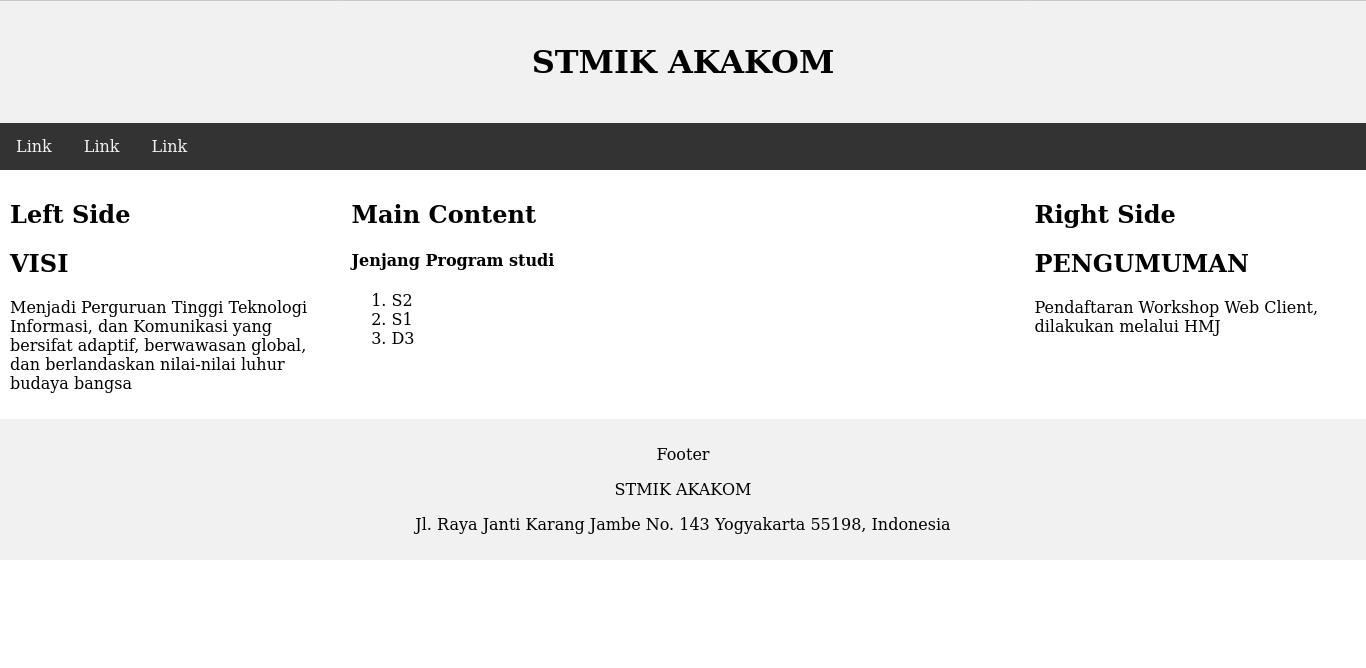
\includegraphics[width=\linewidth]{1.png}
\end{center}

\subsection{Latihan}
\subsubsection{Latihan 1}
Latihan pertama adalah memodifikasi file css pada praktik agar bordernya terlihat.\\
Agar semua border di halaman terlihat, kita tambahkan border-style.\\
Untuk menampilkan border dengan model dotted maka CSS nya seperti berikut:\\
\begin{lstlisting}
* {
    box-sizing: border-box;
    border-style: dotted;
}
\end{lstlisting}
\begin{center}
    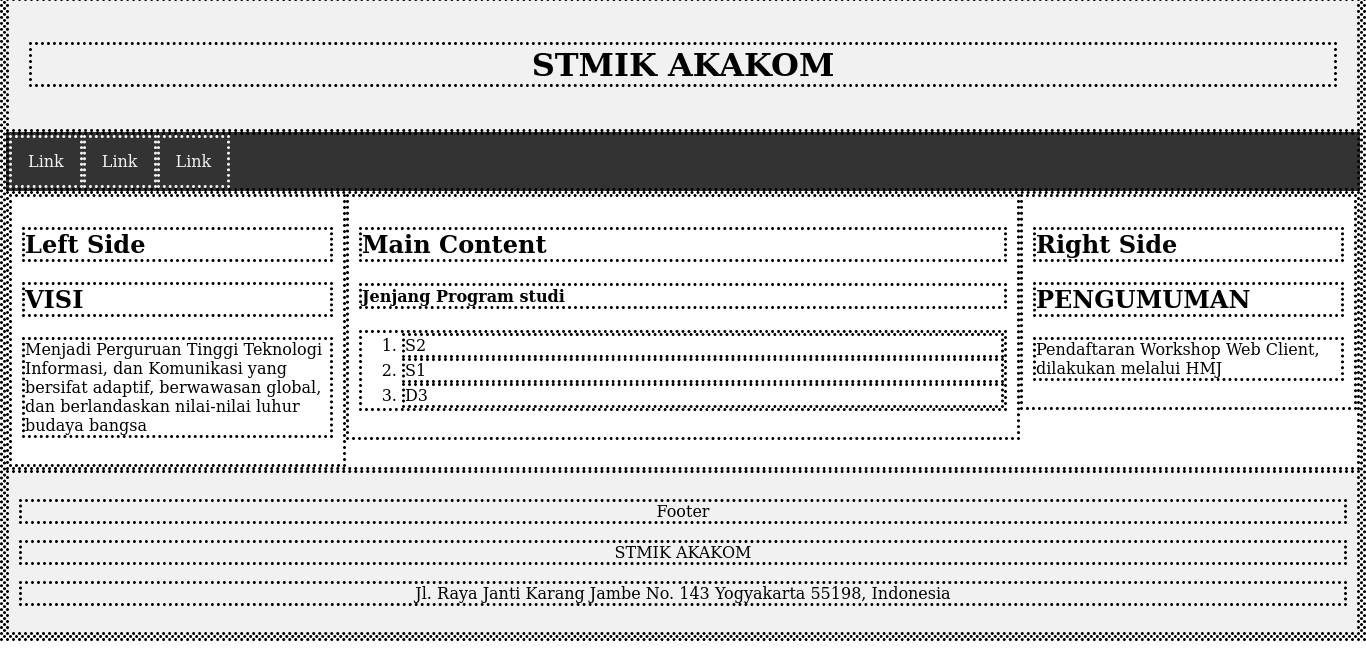
\includegraphics[width=\linewidth]{2.png}
\end{center}

Untuk menampilkan border dengan model solid maka CSS nya seperti berikut:\\
\begin{lstlisting}
* {
    box-sizing: border-box;
    border-style: solid;
}
\end{lstlisting}
\begin{center}
    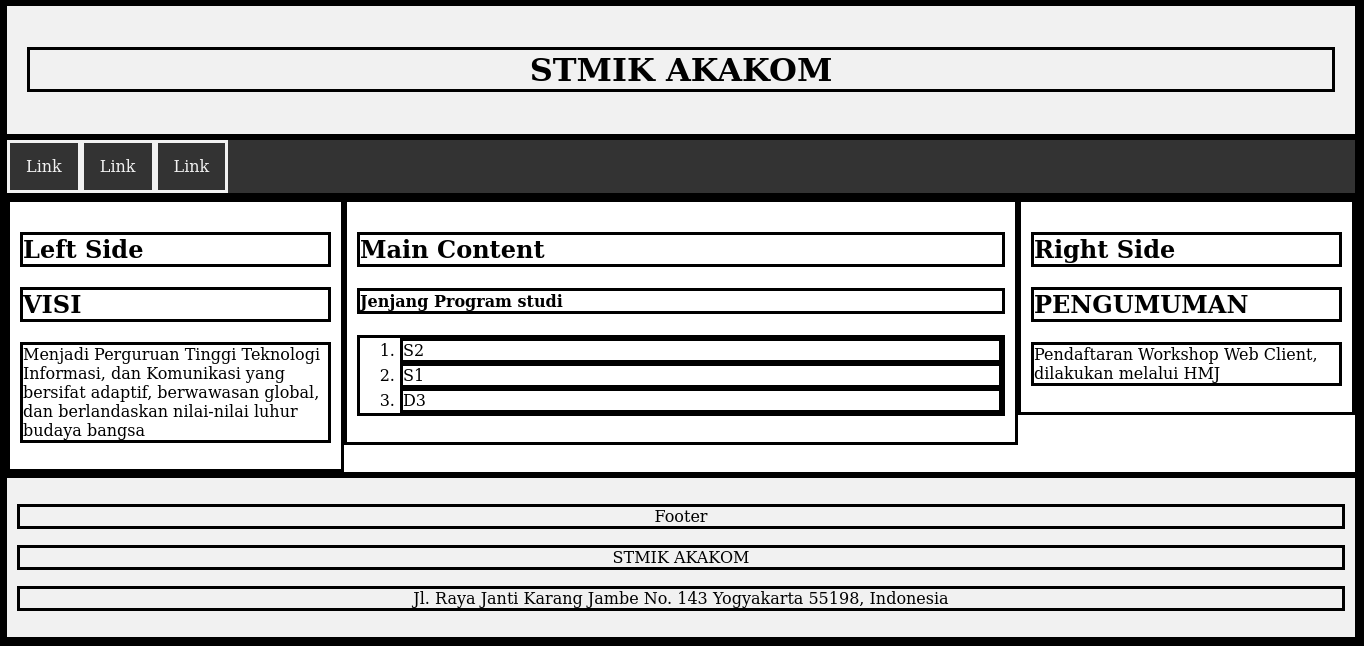
\includegraphics[width=\linewidth]{3.png}
\end{center}

Untuk menampilkan border dengan model dashed maka CSS nya seperti berikut:\\
\begin{lstlisting}
* {
    box-sizing: border-box;
    border-style: dashed;
}
\end{lstlisting}
\begin{center}
    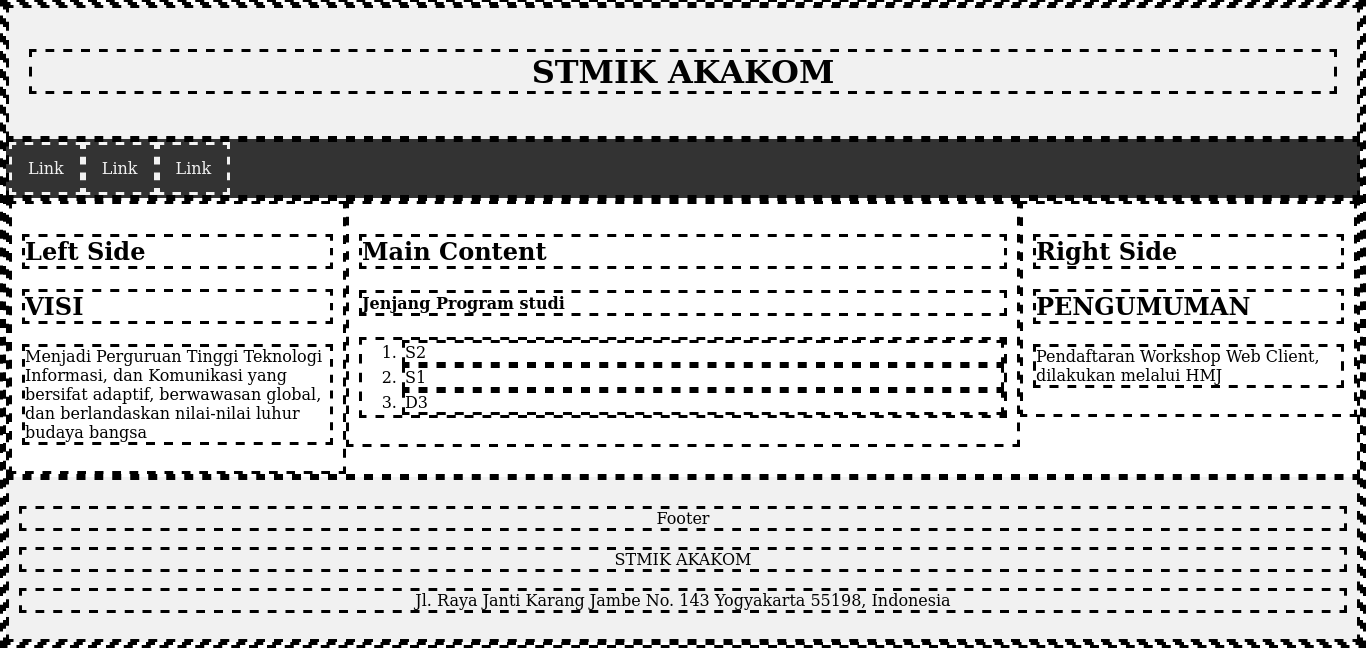
\includegraphics[width=\linewidth]{4.png}
\end{center}

\subsubsection{Latihan 2}
Latihan 2 adalah menambahkan kolom di bagian kanan halaman, dan mengaturnya sehingga tetap proposional.\\
Untuk menambahkan kolom pada bagian kanan tambahkan baris html berikut setelah bagian <div> kolom pengumumunan.
\begin{lstlisting}
<div class="column-side">
    <h2>Latihan</h2>
    <h2>Ini Latihan</h2>
    <p>Latihan Praktikum 4</p>
</div>
\end{lstlisting}
Lalu agar halamannya proposional ganti lebar class column.middle pada file CSS menjadi 25\%.
\begin{lstlisting}
.column.middle {
    width: 25%;
}
\end{lstlisting}
Sehingga jika file html dibuka di browser tampilannya seperti berikut:
\begin{center}
    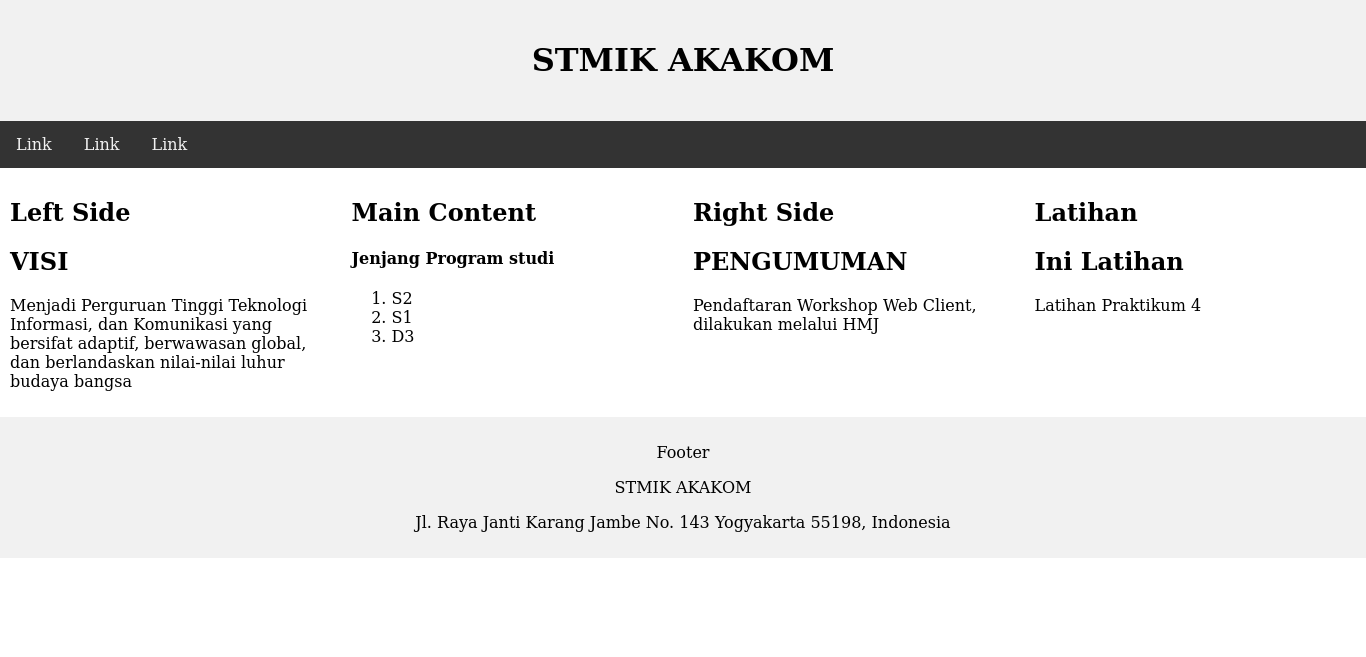
\includegraphics[width=\linewidth]{5.png}
\end{center}

\subsection{Tugas}
Untuk tugas adalah mengisi link pada navigasi sehingga bisa membuka halaman lain.\\
Pertama buat file html yang akan menjadi halaman rujukan pada tombol navigasi.\\
Setelah itu masukkan file html yang sudah ditulis ke dalam tag <a>
\begin{lstlisting}
<a href="index.html">Beranda</a>
<a href="berita.html">Berita</a>
<a href="daftar.html">Pendaftaran</a>
<a href="agenda.html">Agenda</a>
\end{lstlisting}
Tampilan beranda seperti berikut:\\
\begin{center}
    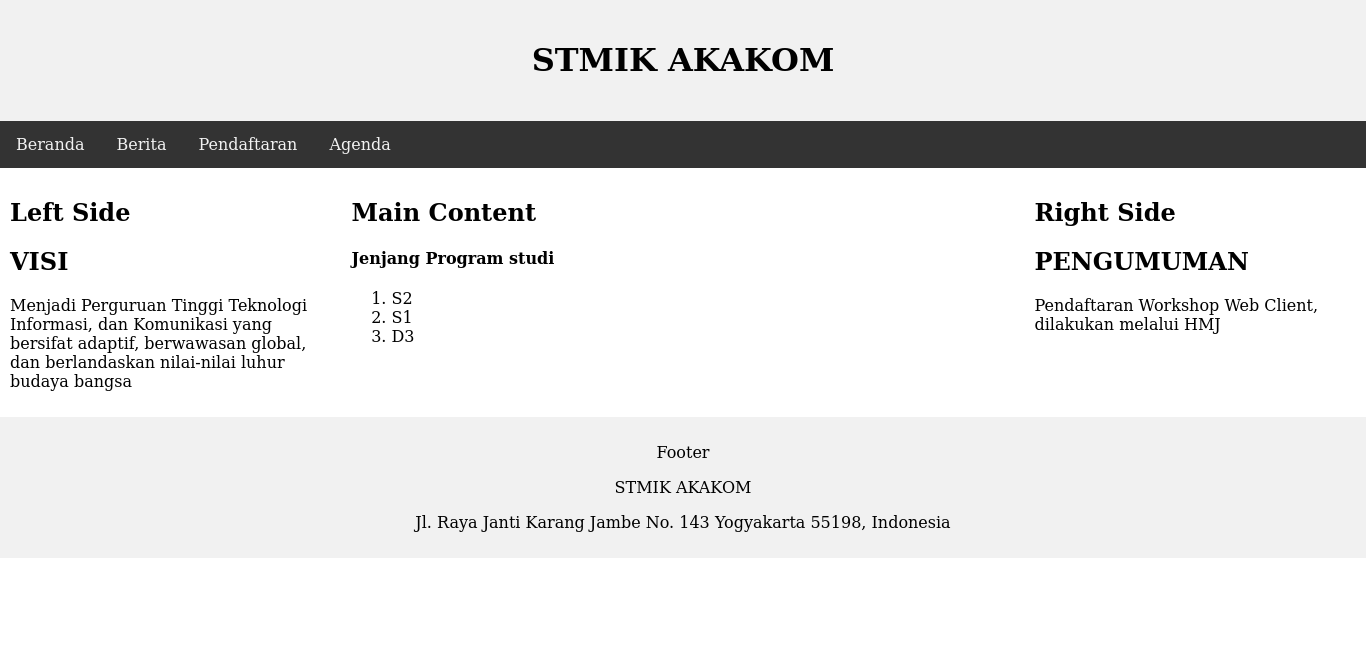
\includegraphics[width=\linewidth]{6.png}
\end{center}
Link Berita yang merujuk ke file berita.html
\begin{center}
    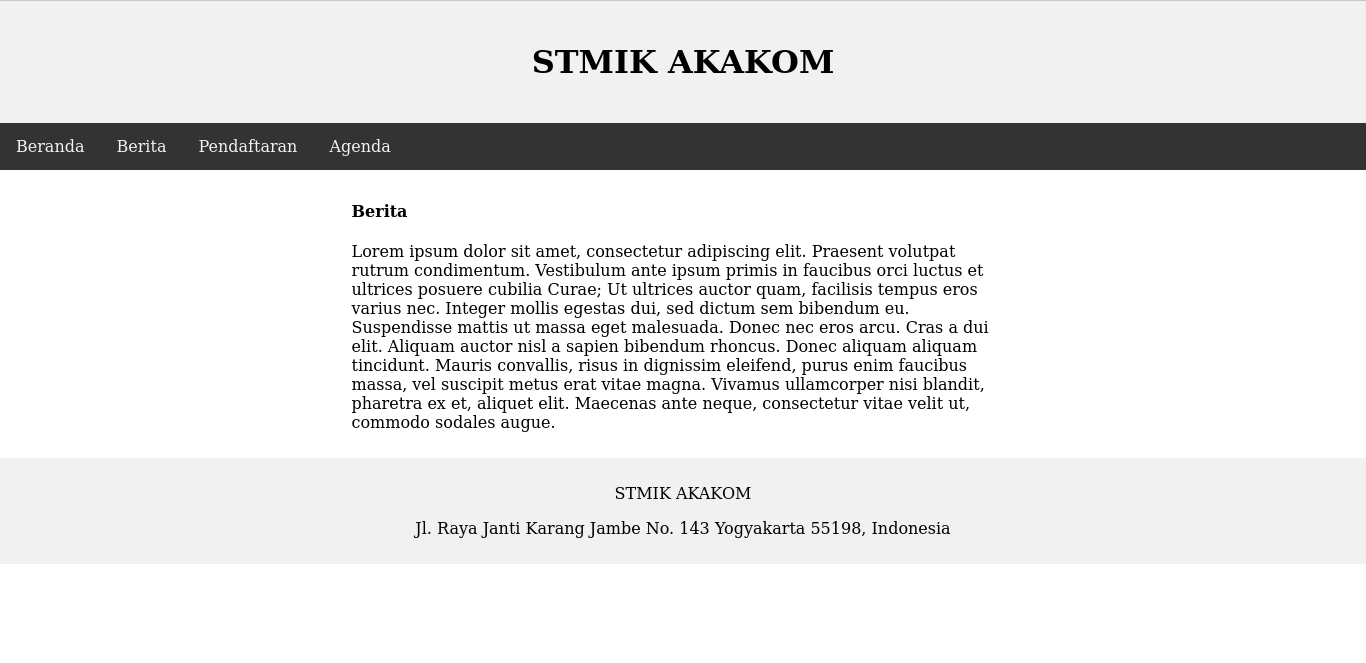
\includegraphics[width=\linewidth]{7.png}
\end{center}
Link Pendaftaran yang merujuk ke file daftar.html
\begin{center}
    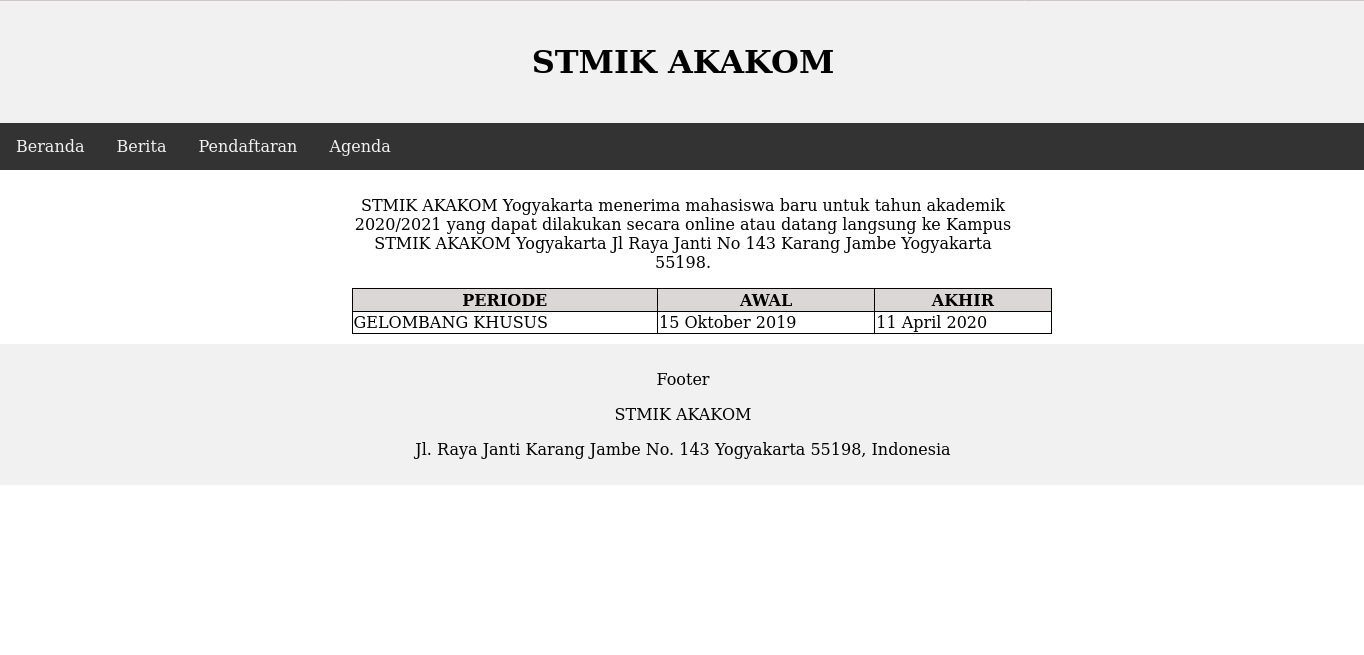
\includegraphics[width=\linewidth]{8.png}
\end{center}
Link Agenda yang merujuk ke file agenda.html
\begin{center}
    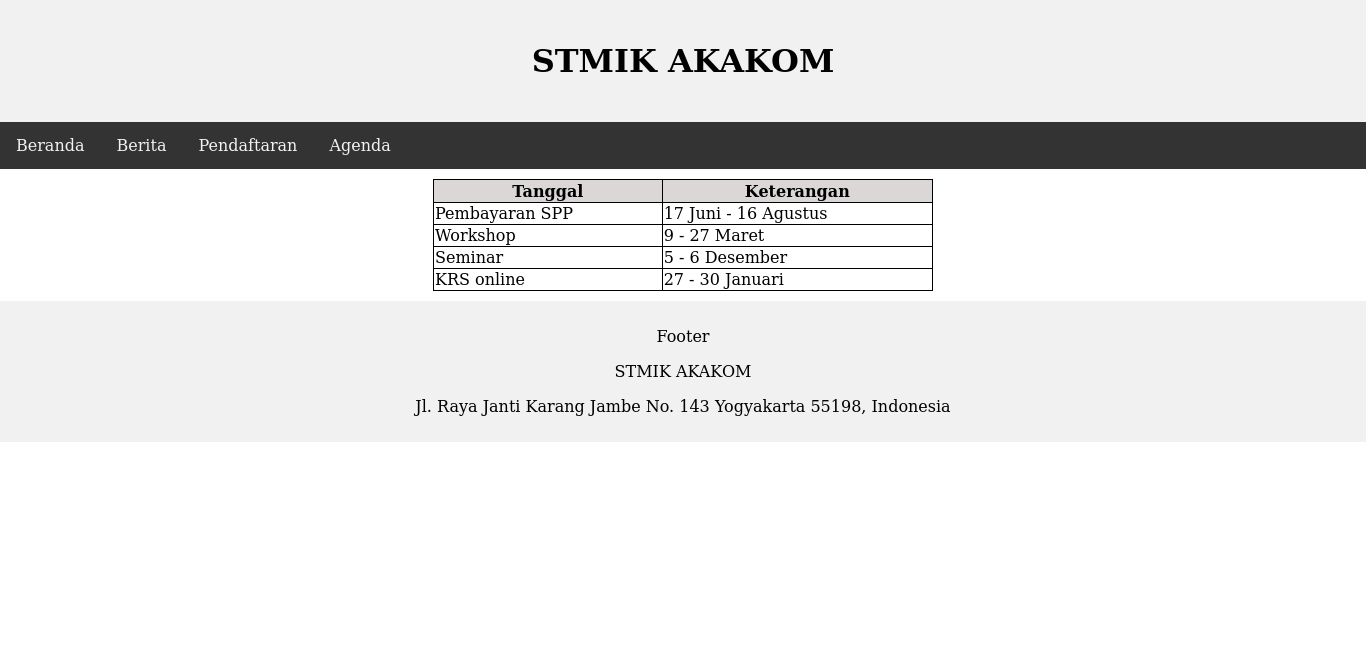
\includegraphics[width=\linewidth]{9.png}
\end{center}
Untuk mengatur tabel tersebut file css ditambahkan baris berikut:
\begin{lstlisting}
table, th, td {
  border: 1px solid black;
  border-collapse: collapse;
}
table {
    margin: 0 auto;
}
th {
    background-color: #dbd7d7;
}
td {
    background-color: #ffffff;
}
\end{lstlisting}


\newpage
\section{Kesimpulan}
Setelah praktik mahasiswa mampu menuliskan konten teks, memformat konten teks dengan CSS (warna, bentuk dan jenis huruf, latar belakang),
mengatuur margin, paadding dan border, positioning konten
\end{document}
